\documentclass[crop=false]{standalone}
%\documentclass{standalone}
\usepackage{tikz} % To generate the plot from csv
\usepackage{pgfplots}
\usepackage{graphicx}
\usepackage{booktabs}
\usepackage{subfig}
\usepackage{float}
\usepackage[section]{placeins} % getting figures below sections
\usepackage{blindtext}
\usepackage{siunitx}
\usepgfplotslibrary{units} % Allows to enter the units nicely
\usetikzlibrary{external} %https://tex.stackexchange.com/questions/1460/script-to-automate-externalizing-tikz-graphics
\tikzexternalize[prefix=savedfigures/]

\pgfplotsset{compat=newest} % Allows to place the legend below plot
\usepackage{pgfplotstable}
\usepgfplotslibrary{statistics}

% #################### Function definition for box plots read table ##################\
\makeatletter
\pgfplotsset{
	boxplot prepared from table/.code={
		\def\tikz@plot@handler{\pgfplotsplothandlerboxplotprepared}%
		\pgfplotsset{
			/pgfplots/boxplot prepared from table/.cd,
			#1,
		}
	},
	/pgfplots/boxplot prepared from table/.cd,
	table/.code={\pgfplotstablecopy{#1}\to\boxplot@datatable},
	row/.initial=0,
	make style readable from table/.style={
		#1/.code={
			\pgfplotstablegetelem{\pgfkeysvalueof{/pgfplots/boxplot prepared from table/row}}{##1}\of\boxplot@datatable
			\pgfplotsset{boxplot/#1/.expand once={\pgfplotsretval}}
		}
	},
	make style readable from table=lower whisker,
	make style readable from table=upper whisker,
	make style readable from table=lower quartile,
	make style readable from table=upper quartile,
	make style readable from table=median,
	make style readable from table=average,
	make style readable from table=lower notch,
	make style readable from table=upper notch
}
\makeatother
\begin{document}

\section{5 2 Mumford0 GA Mut threshold 20210721 225748}

% ######################## UTRP GA Mutation threshold ######################## 
\begin{figure} 
\centering 
\tikzsetnextfilename{UTRP_NSGAII_BP_mut_threshold_phd} 
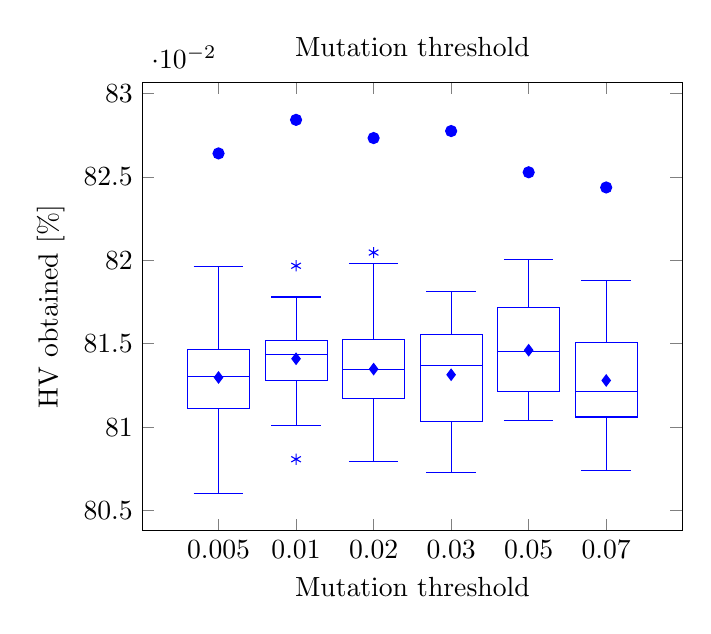
\begin{tikzpicture} 
\begin{axis}[ 
title={Mutation threshold}, 
boxplot/draw direction=y, 
xtick={1,2,3,4,5,6}, 
xticklabels={0.005,0.01,0.02,0.03,0.05,0.07}, 
x tick label style={rotate=0, align=center}, 
xlabel={Mutation threshold}, 
scaled y ticks={base 10:2}, %y tick label style={/pgf/number format/.cd,fixed,precision=3, zerofill}, 
ylabel={HV obtained [\%]}, 
] 

% ############## Mut_threshold=0.005 ################## 
\addplot[boxplot, mark=asterisk, 
boxplot prepared={ 
lower whisker=0.80603, 
upper whisker=0.81964, 
lower quartile=0.81112, 
upper quartile=0.81466, 
median=0.81304, 
average=0.81298}, 
color = blue, solid, area legend] 
coordinates {}; 
\addplot[only marks,mark=*,color = blue]coordinates{(1,0.8264)}; 

% ############## Mut_threshold=0.01 ################## 
\addplot[boxplot, mark=asterisk, 
boxplot prepared={ 
lower whisker=0.81009, 
upper whisker=0.8178, 
lower quartile=0.81282, 
upper quartile=0.81518, 
median=0.81437, 
average=0.8141}, 
color = blue, solid, area legend] 
coordinates {
(2,0.80808)
(2,0.81967)}; 
\addplot[only marks,mark=*,color = blue]coordinates{(2,0.82841)}; 

% ############## Mut_threshold=0.02 ################## 
\addplot[boxplot, mark=asterisk, 
boxplot prepared={ 
lower whisker=0.80795, 
upper whisker=0.81979, 
lower quartile=0.81173, 
upper quartile=0.81526, 
median=0.81346, 
average=0.81348}, 
color = blue, solid, area legend] 
coordinates {
(3,0.82046)}; 
\addplot[only marks,mark=*,color = blue]coordinates{(3,0.82732)}; 

% ############## Mut_threshold=0.03 ################## 
\addplot[boxplot, mark=asterisk, 
boxplot prepared={ 
lower whisker=0.80731, 
upper whisker=0.81814, 
lower quartile=0.81034, 
upper quartile=0.81554, 
median=0.81369, 
average=0.81314}, 
color = blue, solid, area legend] 
coordinates {}; 
\addplot[only marks,mark=*,color = blue]coordinates{(4,0.82774)}; 

% ############## Mut_threshold=0.05 ################## 
\addplot[boxplot, mark=asterisk, 
boxplot prepared={ 
lower whisker=0.81039, 
upper whisker=0.82006, 
lower quartile=0.81213, 
upper quartile=0.81716, 
median=0.81453, 
average=0.81461}, 
color = blue, solid, area legend] 
coordinates {}; 
\addplot[only marks,mark=*,color = blue]coordinates{(5,0.82527)}; 

% ############## Mut_threshold=0.07 ################## 
\addplot[boxplot, mark=asterisk, 
boxplot prepared={ 
lower whisker=0.80743, 
upper whisker=0.81877, 
lower quartile=0.81061, 
upper quartile=0.81509, 
median=0.81212, 
average=0.8128}, 
color = blue, solid, area legend] 
coordinates {}; 
\addplot[only marks,mark=*,color = blue]coordinates{(6,0.82436)}; 

\end{axis}
\end{tikzpicture}
\end{figure} 
\begin{table}
\centering
\caption{Legend for the boxplot.}
\begin{tabular}{ll}
\toprule
 Index &  Name \\
\midrule
     0 & 0.070 \\
     1 & 0.050 \\
     2 & 0.030 \\
     3 & 0.020 \\
     4 & 0.010 \\
     5 & 0.005 \\
\bottomrule
\end{tabular}
\end{table}

\end{document}
